\documentclass[a4paper, british]{article}

\usepackage[utf8]{inputenc}
\usepackage[T1]{fontenc}
\usepackage{babel}
% \usepackage[margin=2.5cm,a4paper]{geometry}
% \usepackage[skip=1em]{parskip}
\usepackage{lmodern} 
\usepackage{microtype}
% \usepackage{xcolor}
\usepackage{graphicx}
\graphicspath{ {./figures/} }
\usepackage{float}
\usepackage{adjustbox} % rescale - useful for Dia exported TeX
\usepackage{tikz}
% \usepackage{pgfplots}
\usepackage{booktabs} %tables no vertical lines
\usepackage{enumitem}
% \usepackage{array}
% \usepackage{authblk}
% \usepackage{fancyhdr} %headers and footers
% \usepackage{titlesec}
% \usepackage{tcolorbox} % framed text boxes
\usepackage{mathtools, amssymb, amsthm}
% \usepackage{gensymb}
\usepackage{lineno}
\usepackage{minted} % code highlighting
\usepackage{chemformula} % chemical formulae
\usepackage{chemfig} % molecular figures
\usepackage{siunitx}
\usepackage{csquotes}
\usepackage[titletoc, title]{appendix}
% \usepackage{lettrine} % initials

\usepackage[
pdfauthor={Adam Menne},
pdftitle={Applied Mathematics - Assignment 3},
pdfsubject={},
pdfkeywords={}]{hyperref}

\usepackage[noabbrev]{cleveref}

\usepackage[
backend=biber,
style=numeric,
sorting=none,
doi=true,
isbn=false
]{biblatex}
\addbibresource{citations.bib}

\setlength{\parskip}{1em}
\setlength{\parindent}{0em}
\linespread{1.3}

\usemintedstyle[julia]{xcode}

\title{Applied Mathematics - Assignment 3}
\date{Last edited on \today}
\author{Adam Menne -- 24942901\\ Stellenbosch University}

\begin{document}

\maketitle

\vspace{40mm}

\tableofcontents

\newpage

\section{Problem 1}


\subsection*{(a), (b), (c)}

\begin{listing}[H]
    \begin{minted}[linenos, gobble = 2, frame = leftline, framesep = 2mm]{julia}
    function euler(f, u0, tspan, h)
        n = abs(-(tspan...)) / h
        collect(
            begin
                u0 += h * f(u0); u0
            end
            for t in tspan[1]:n
        )
    end   
    \end{minted}
    \caption{Euler's Method}
    \label{lst:euler}
\end{listing}

\begin{listing}[H]
    \begin{minted}[linenos, gobble = 2, frame = leftline, framesep = 2mm]{julia}
    function f!(u)
        du1 = 4*u[1] + 2*u[2]
        du2 = 3*u[1] + 3*u[2]
        return [du1, du2]
    end
    \end{minted}
    \caption{The differential equation}
    \label{lst:dif_func}
\end{listing}

\begin{listing}[H]
    \begin{minted}[linenos, gobble = 2, frame = leftline, framesep = 2mm]{julia}
    euler(f, [10.0; -5.0], (0.0, 0.5) 0.01)
    \end{minted}
    \caption{Calling the function}
    \label{lst:func_call}
\end{listing}

\begin{figure}[H]
    \centering
    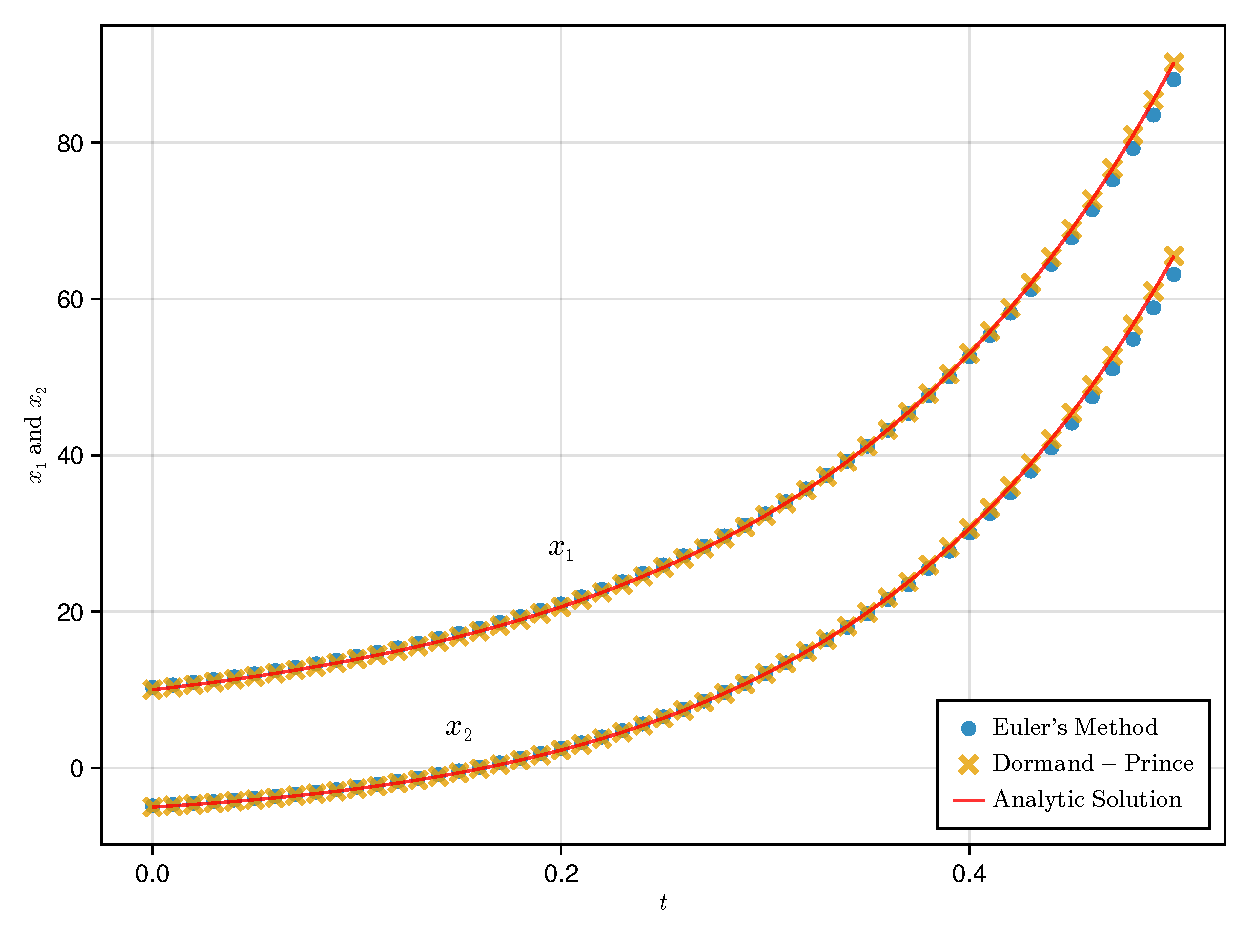
\includegraphics[width=\textwidth]{figures/f1.pdf}
    \caption{Comparison of numeric to analytic solutions}
    \label{fig:1}
\end{figure}



\subsection*{(d)}

The Dormand-Prince method, which I believe is the default used by the ode45 solver, offered substantially improved accuracy over the Euler method, even though its abilities were stunted by using a fixed step-size. However, it is not as performant as the Tsitouras method used in the other problems in this assignment

\newpage


\section{Problem 2}

\subsection*{(a)}

\(x\) represents the prey, and \(y\) the predator.

\subsection*{(b)}

\begin{figure}[H]
    \centering
    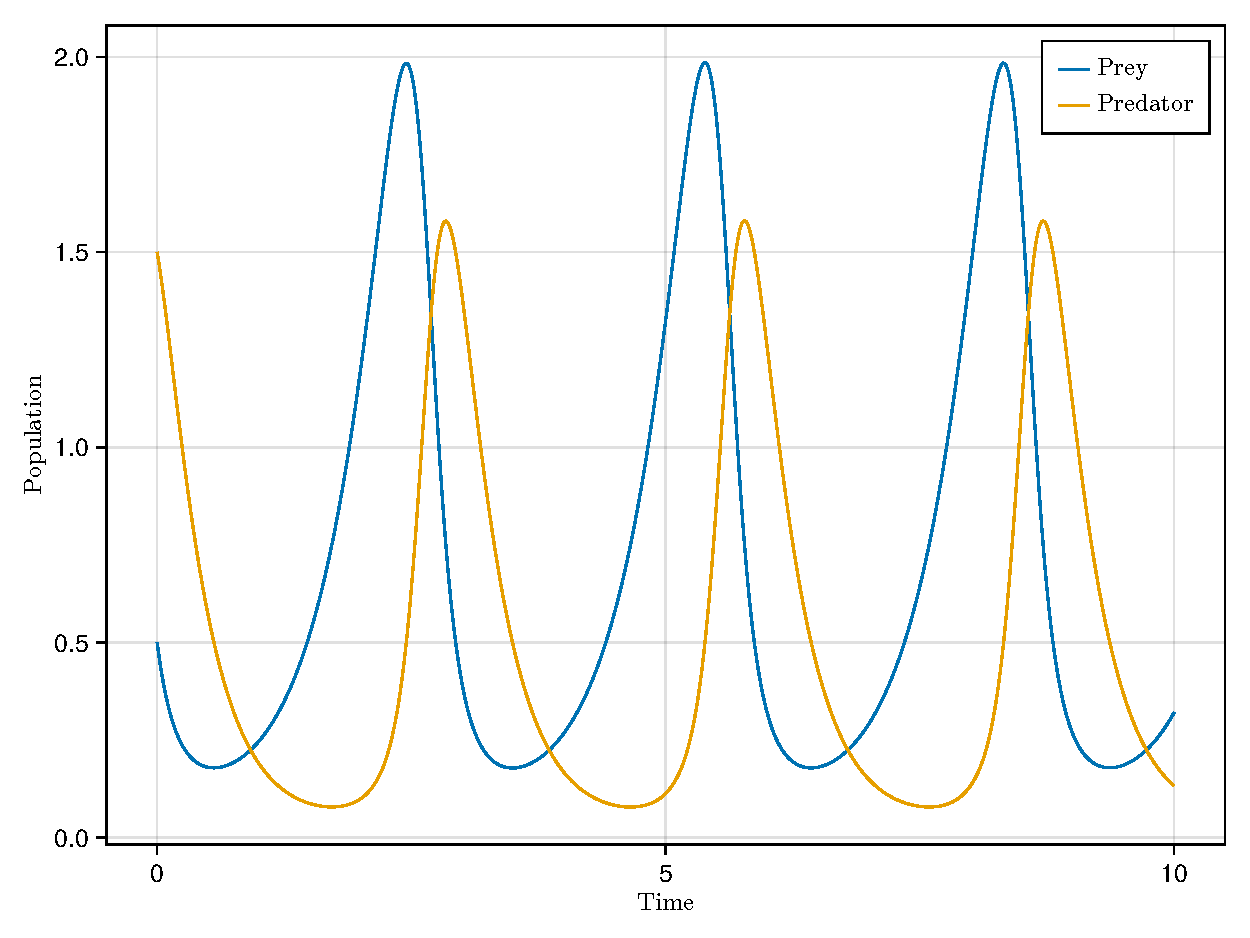
\includegraphics[width=\textwidth]{figures/f2.pdf}
    \caption{Lotka-Volterra predator-prey model over 10 years}
    \label{fig:2}
\end{figure}

\subsection*{(c)}

The populations are first equal at 0.93 days.

The extrema of the prey are 0.178 and 1.99, and the predators 0.0782 and 1.58.

\newpage

\section{Problem 3}

\subsection*{(a)}

\begin{figure}[H]
    \centering
    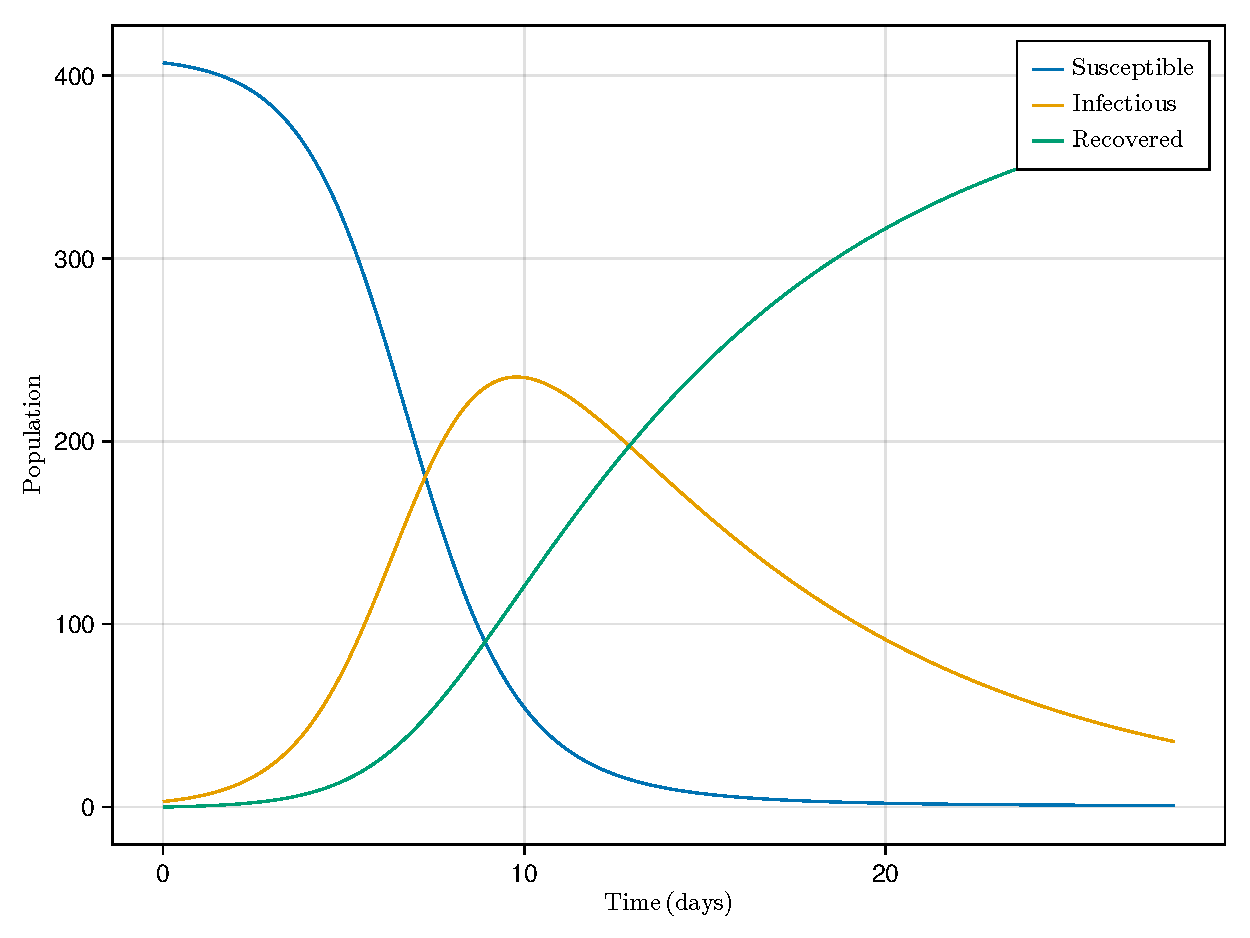
\includegraphics[width=\textwidth]{figures/f3.pdf}
    \caption{SIR model over 4 weeks}
    \label{fig:3}
\end{figure}

\subsection*{(b)}

\subsubsection*{(i)}

235.14

\subsubsection*{(ii)}

35.78

\newpage

\section{Problem 4}

\subsection*{(a)}

With the substitution \(y = x \prime\), we may describe the Van der Pol oscillator with the first-order system:

\begin{align*}
    x \prime &= y \\
    y \prime &= \mu (1 - x^2)y - x
\end{align*}

\subsection*{(b)}

\begin{figure}[H]
    \centering
    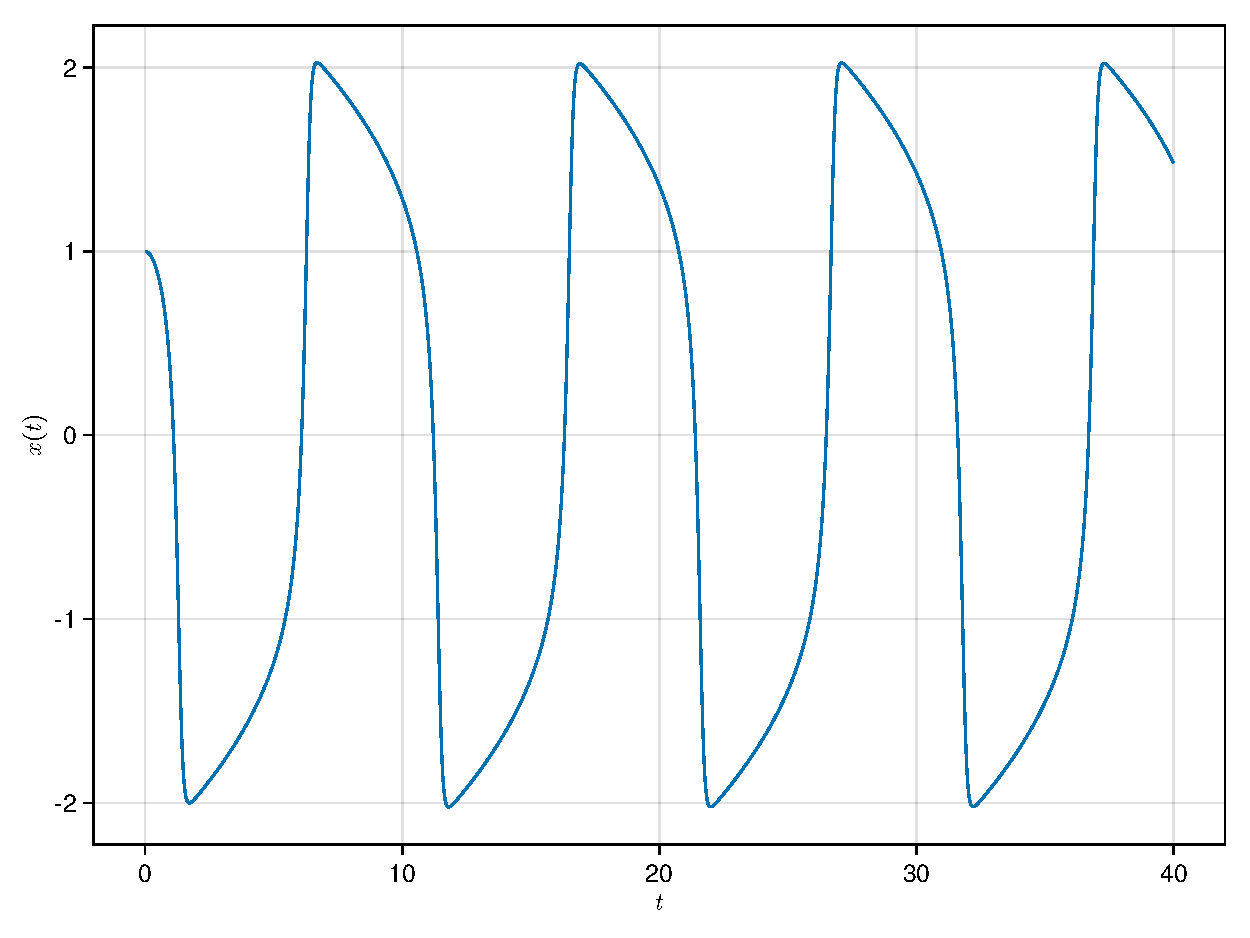
\includegraphics[width=\textwidth]{figures/f4_1.pdf}
    \caption{Solution to the Van der Pol oscillator}
    \label{fig:4_1}
\end{figure}

\subsection*{(c)}

\begin{figure}[H]
    \centering
    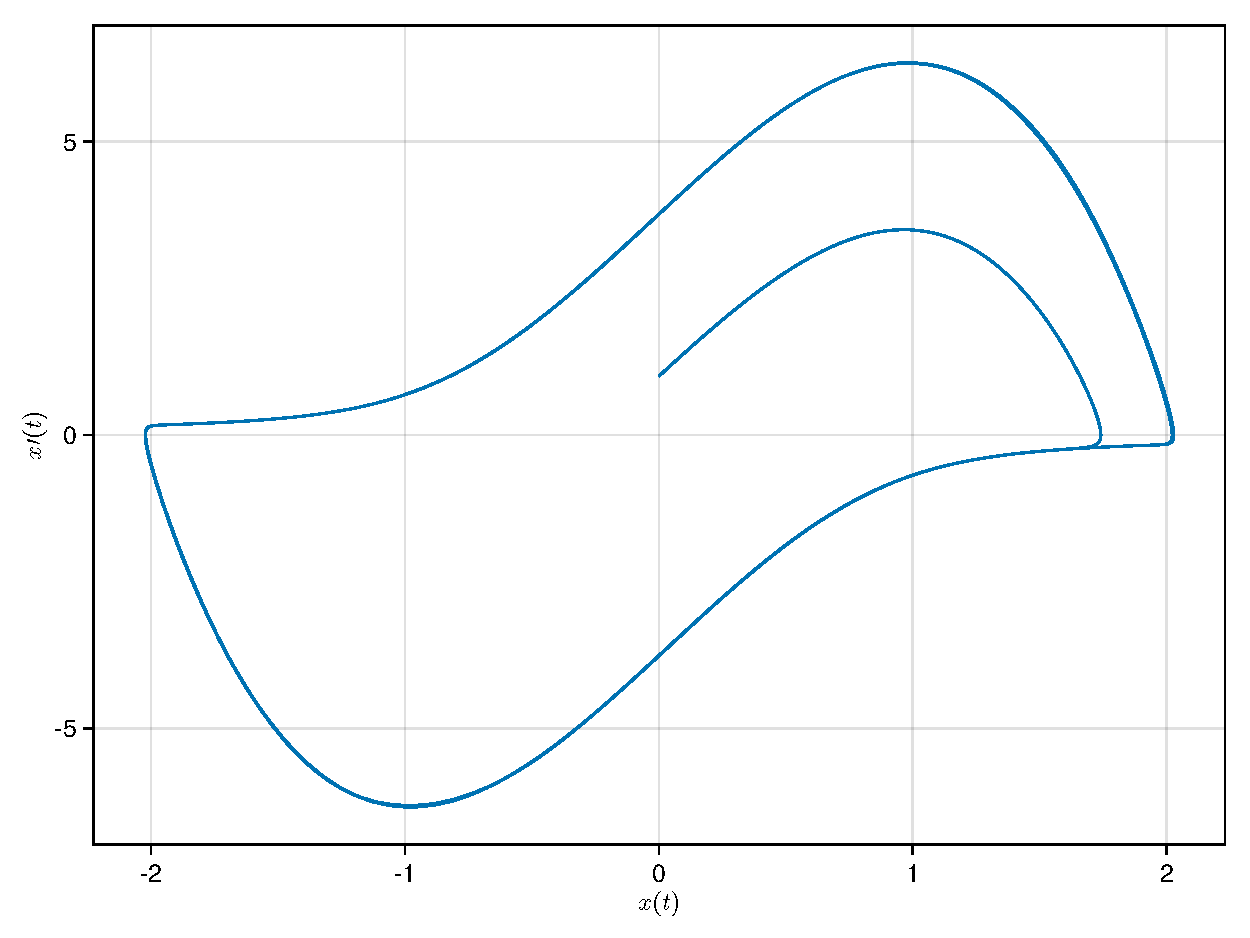
\includegraphics[width=\textwidth]{figures/f4_2.pdf}
    \caption{Phase plot of the Van der Pol oscillator}
    \label{fig:4_2}
\end{figure}

A static export of the notebook containing all analysis and figures is available at \url{https://adammenne.github.io/applied_mathematics_244/assignment_3/notebook.html}.\\ 
With full source code available at \url{https://github.com/AdamMenne/applied_mathematics_244/tree/master/assignment_3}


\end{document}